\subsubsection{Motor- og sensorstyring}
Som set i \ref{sec:Arkitektur} \\
Styringen af de aktuelle motorer/sensorer sker udelukkende via 2 PSoC's: en Master- (MP) og en Slave-PSoC (SP). MP har foruden at yde statusopdateringer til DevKit8000 (DK8k) til opgave at styre motorerne/sensorerne for x-/y-akserne og at sende kommandoer til/modtage status fra SP. SP har til opgave at styre motorerne for z-aksen, skruen og åbningsmekanismen. Som set i sekvensdiagrammet (figur \ref{SD_PSoC})) påbegyndes detektering og åbning af vinflasken ved en kommando fra DK8k til MP, som efter at have fastslået flaskens x- og y-position giver besked til SP om at løfte sensorerne til en position, der er en vis afstand under flaskens top. SP giver besked til MP om, at dette er gjort, hvorefter MP med y-sensoren detekterer, om der står en flaske eller ej. Dette gentages med en position over flaskens top. Herefter flytter MP åbningsmekanismen til en position over flasken, hvorefter der gives besked til SP om at åbne flasken. Når dette er gjort resettes alle relevante komponenter til en startposition, hvorefter proppen disponeres, og der gives besked til DK8k om, at flasken er drikkeklar. \\
Noget, som ikke er vist i sekvensdiagrammet, er fejlscenarier. Disse findes for de metoder, hvor der i diagrammet returneres \textit{SUCCESS}. I disse tilfælde resettes motorerne, og MP sender en statusbesked til DK8k om den pågældende fejl.

\myparagraph{Klasser og funktioner}
Sideløbende med sekvensdiagrammet er følgende klassediagram blevet udformet: (indsæt billede af dette)

De variable i de to Controller-klasser, der ender i \textit{Stop}, repræsenterer trykknapperne. Disse benyttes af Motor-klasserne, når en bestemt position ønskes registreret. Heriblandt start- og slutposition på en gældende akse. \\
Klassernes overordnede funktionalitet burde ud fra deres titler og ovenstående beskrivelse virke forholdsvis indlysende, men visse af metoderne kræver yderligere forklaring.
\\
\\
\textbf{locateX() / locateY()} \\
For nærmere at beskrive disse to metoder, hvis funktionalitet ikke afviger fra hinanden, er følgende aktivitetsdiagram blevet udarbejdet: \\

\begin{figure}[H]
	\centerline{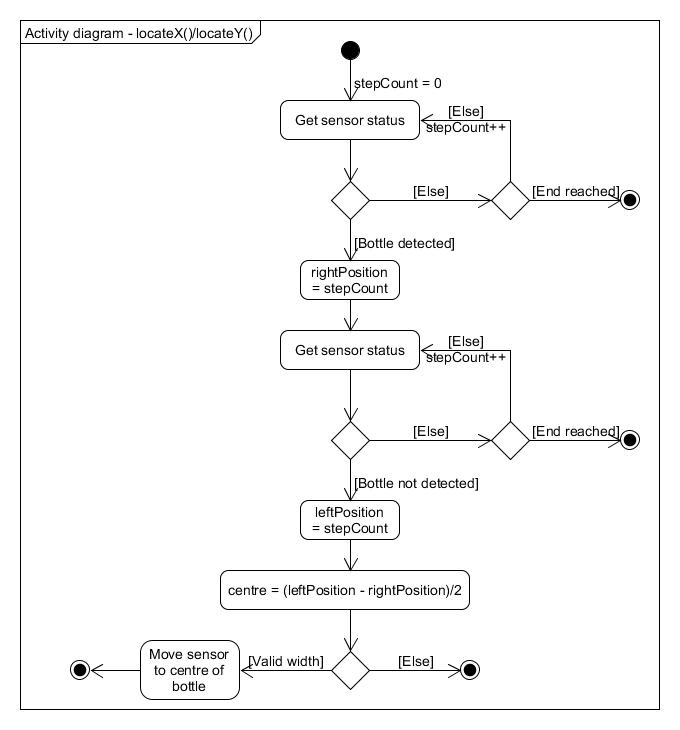
\includegraphics[scale=0.5]{tex/Design/PSoC/AD_locate.jpg}}
	\caption{Aktivitetsdiagram over locateX()/locateY()}
	\label{AD_locate}
\end{figure}

Ved indtrædelse i metoden nulstilles en tæller \textit{stepCount}, som tæller antallet af steps taget. Derefter måles med sensor, om en flaske er registreret. Så længe dette ikke er tilfældet, skal motoren fortsat køre, og \textit{stepCount} skal tælles op. I så fald enden på aksen nås, skal metoden afslutte og returnere en fejlværdi. Hvis flasken registreres, gemmes \textit{stepCount} i \textit{rightPosition}. Der fortsættes efter samme mønster, indtil der ikke længere registreres en flaske, eller enden er nået. Hvis førstnævnte er tilfældet, gemmes \textit{stepCount} i \textit{leftPosition}, hvorefter afstanden til flaskens midte beregnes ud fra \textit{rightPosition} og \textit{leftPosition}. Denne værdi sammenlignes med en forudbestemt værdi for at sikre, at det er en kompatibel flaske, der er indsat. Hvis ikke, afsluttes metoden og returnerer en fejlværdi. Ellers flyttes sensoren til flaskens midte, og metoden returnerer en succesværdi.
\\
\\
\textbf{Øvrige metoder}

\textbf{positionZ(uint8)} løfter sensorerne et vist antal steps, som er bestemt ud fra det medgivne argument, op fra startpositionen.

\textbf{confirmHeight(uint8)} skal registrere med y-sensoren om en flaske kan registreres i den givne højde alt efter den medgivne parameter (UNDER\_TOP: flaske skal registreres, ABOVE\_TOP: flaske skal ej registreres).

\textbf{positionXY()} skal ud fra forudbestemte værdier køre motorerne et vis antal steps mod åbningsmekanismens centrum.

\textbf{reset()} kører motorerne indtil deres  respektive trykknap ved startpositionen er påtrykt.

\textbf{openBottle()} skal få z-motorerne til at presse åbningsmekanismen ned mod vinflasken ud fra et forudbestemt antal steps, hvorefter s-motoren skal sætte skruen til at dreje et bestemt antal steps, så p-motoren kan hive i proppen, indtil den rammer en trykknap.

\textbf{dispose()} skal blot dreje s-motoren et vis antal steps for at disponere proppen.